\documentclass[12pt]{article}
\usepackage{xparse}
\usepackage[utf8]{inputenc}
\usepackage{graphicx}
\usepackage{amsmath}
\usepackage{calligra}
\usepackage{asymptote}
\usepackage[version=4]{mhchem}
\usepackage{titlesec}
\setcounter{secnumdepth}{4}
\titleformat{\section}[block]{\sffamily\Large\filcenter\bfseries}{\thesection.}{0.25cm}{\Large}
\titleformat{\subsection}[block]{\large\bfseries\sffamily}{\thesubsection.}{0.2cm}{\large}
\titleformat{\subsubsection}[block]{\small\sffamily}{\thesubsubsection}{0.18cm}{\large}


\usepackage{enumitem}

\newcommand{\scriptr}{\mathcalligra{r}\,}
\newcommand{\boldscriptr}{\pmb{\mathcalligra{r}}\,}
\usepackage{physics}
\usepackage{tcolorbox}
\usepackage{tikz}
\usepackage[a4paper]{geometry}
\usepackage{hyperref}
\title{\sffamily{MM 209 Notes}}
\author{\sffamily{\color{blue}{Advait Risbud}}}
\date{May 21'}

\begin{document}
	\sffamily
	\maketitle
	\tableofcontents
	\pagebreak
\section{Introduction}
	Energy is the ability to bring about desired changes in materials. Thermodynamics allows us to predict the properties that a system will exhibit. We can proceed with determining the properties of the system in 2 ways:
	\begin{itemize}
		\item Determine the behaviour of each particle in the system.
		\item Determine a quantity that represents the average properties of that system.
	\end{itemize}
	\textit{Classical thermodynamics} treats systems as a continuum and ignores the microscopic properties of the system(includes the first and second law of thermodynamics). \textit{Statistical thermodynamics} arrives at results for macroscopic systems from an atomistic point of view using ideas from quantum mechanics and statistical mechanics. \textit{Irreversible thermodynamics} talks about the properties of irreversible processes. 
	
	\subsection{Terminology}
	\begin{itemize}
		\item System: The subject of the analysis. It is the macroscopically identifiable collection of matter on which we will focus our attention.
		\item Surrounding: The rest of the universe close to the system such that it has a perceptible effect on the system is called the surrounding.
		\item Boundary: The surface which separates the system and the surrounding is called the boundary.
	\end{itemize}
    
    There can be two types of exchanges between system and surrounding, energy and matter. Thermal energy while being transferred is referred to as \textit{heat}. So we classify systems as follows \footnote[1]{Refer Gaskell}:
    \begin{enumerate}
    	\item Isolated systems : In these systems, no work is done on or by the system. In addition,
    	energy or matter may not enter or leave it(adiabatic and impermeable). Thus, the energy of these systems
    	remains constant, as does the overall composition. Isolated systems are therefore
    	unaffected by changes in the surroundings.
    	
    	\item Closed systems : These are systems which may receive (or give off) energy from
    	(or to) the surroundings. The boundaries are called diathermal ; that is, they allow
    	thermal energy to transfer through them into or out of the system. However, the boundaries are impermeable to matter(diathermic); hence, the amount of matter is constant in
    	these systems.
    	
    	\item Open systems : These are systems which can exchange both energy and matter with
    	the surroundings(diathermic and permeable). Neither the energy nor the composition of these systems need
    	remain constant. The boundaries are both permeable and diathermal.
    \end{enumerate}

        Beyond this we clarify systems based on number of phases, components and reacting/non-reacting nature of the system. \\
        
        Intensive properties are those which do not depend on the mass of the system whereas extensive properties depend on the mass of the system. Examples of intensive properties are density, specific heat, ionisation energy per mole etc. Examples of extensive properties are enthalpy, entropy, internal energy.\\
        
        \subsection{State Functions}
        Since it is difficult to know the properties of each particle in the system, classical thermodynamics uses a few thermodynamic variables to define the \textit{macroscopic state} of the system. It is found that the values of only two independent thermodynamic variables need to be known after which the state gets fixed. This is called the Duhem Postulate.
        State functions are those properties that do not depend on the history of the system. Which means that two systems in the same state will have the same value of that property irrespective of which process brought them to that state. Those properties that depend on the path followed by the system are called path functions. In case of an ideal gas we have the relation $PV=nRT$. So consider a 3 dimensional P-V-T plot and in that take a small change in volume $dV$
        \begin{equation}
        	dV=\Bigg(\pdv{V}{P}\Bigg)_T dP+\Bigg(\pdv{V}{T}\Bigg)_P dT \label{1}
        \end{equation}
       
        If V is a state function i.e. a function of only P and T then \eqref{1} should be a perfect differential. Which means that the differential form should be closed which implies it is exact since our domain is convex. Therefore
        \begin{equation}
        	\pdv{T}\Bigg(\pdv{V}{P}\Bigg)=\pdv{P}\Bigg(\pdv{V}{T}\Bigg) \quad \qq{(put V=nRT/P)}
        \end{equation}
        
        All state functions are exact differentials. Consider the coefficient of $dP$ in \eqref{1}. It is the change of volume per unit pressure. When divided by volume it's magnitude is nothing but the isothermal compressibility of the substance $\beta$. The coefficient of $dT$ is change in volume per unit change in temperature which when divided by volume is nothing but the isobaric coefficient of thermal expansion $\alpha$.
        \begin{align}
        	\beta&=-\frac{1}{V}\Bigg(\pdv{V}{P}\Bigg)_T \\
        	\alpha &=\frac{1}{V}\Bigg(\pdv{V}{T}\Bigg)_P
        \end{align} 
    
       Therefore \eqref{1} becomes
       \begin{equation}
       	dV=\alpha V dP-\beta V dT
       \end{equation}
       
       \subsubsection{Reciprocity theorem}
       This a property of partial derivatives of state functions, which in case of thermodynamics are P, V and T. Let $x=X(y,z)$, we have
       \begin{equation}
       	\Bigg(\pdv{y}{x}\Bigg)_z=\dfrac{1}{(\pdv{x}{y})_z}
       \end{equation}
       which gives us 
       \begin{equation}
       	\Bigg(\pdv{x}{y}\Bigg)_z\times \Bigg(\pdv{y}{z}\Bigg)_x\times \Bigg(\pdv{z}{x}\Bigg)_y=-1
       \end{equation}
   \pagebreak
\section{Conjugate Variables}
   All thermodynamic variables are expressed in terms of conjugate variables. In classical mechanics a small increment in force gives rise to a small displacement which has a corresponding energy increment. Akin to this in thermodynamics a generalised force gives rise to a generalised displacement which cause a change in the thermodynamic potential(energy) of the system. 
   \begin{center}
   	\begin{tabular}{|c | c | c ||} 
   		\hline
   		System & Generalised force & Generalised disp.  \\ [0.5ex] 
   		\hline\hline
   		Fluid & Pressure(P) & Volume(V) \\ 
   		\hline
   		String & Tension(T) & Length(L) \\
   		\hline
   		Surface & Surface Tension($\sigma$) & Area(A)  \\
   		\hline
   		All Systems & Temperature(T) & Entropy(S) \\
   		\hline
   		Magnetic & Magnetic field(B) & Dipole moment(m) \\ [1ex] 
   		\hline
   	\end{tabular}
   \end{center}
    
    
    The thermodynamic force is always an intensive variable and the displacement is always an extensive variable, yielding an extensive energy transfer. The intensive (force) variable is the derivative of the internal energy with respect to the extensive (displacement) variable, while all other extensive variables are held constant\footnote[2]{Wikipedia: Conjugate variables}. \\
    
    A process which can be reversed at any point by a slight change in the magnitude of the driving force is called a reversible process. Reversible processes must be quasi-static which means that they must "almost" be in equilibrium at every state. So reversible processes are much slower than irreversible processes. An example is the compression of a piston. If a piston is compressed very slowly while maintaining equilibrium at every step, the piston can be pulled out just as slow and all the energy that was imparted during compression can be retained. Whereas if we push the piston in very fast, sound waves can be generated and pulling the piston back out will not give back the energy that was lost through sound waves as the waves might escape the system. \\
    
    A reversible process must not have hysteresis. Hysteresis means that the process should follow the same path on being reversed. An example of a reversible process is loading and unloading of a rod when stress is applied below the yield stress. When applied stress is more than the yield stress then plastic deformation takes and when the rod is unloaded it will follow a path parallel to the loading curve. Hence showing hysteresis and so is not a reversible process. \\
    \pagebreak
    
\section{Pure Substances}
    \subsection{What is a pure substance?}
    A substance that has a fixed chemical composition throughout is called a pure substance. Pure elements and compounds are obviously included, even a mixture of elements or compounds is permitted so long as it is homogenous. A mixture of oil and water is not a pure substance as it is not homogenous. A substance can be composed of multiple phases but still be pure provided the compositions of the phases are the same for e.g. liquid air and gaseous air are different phases but will have a different composition due to the varying boiling points of gases in air.\\
    
    A liquid that is not about to vaporise is called a \textbf{sub-cooled liquid} or a \textbf{compressed liquid}. A liquid that is about to vaporise is called a \textbf{saturated liquid}.
\section{Equilibrium}
    In an isolated system there will be no external influences on a system but on an atomistic scale there can still be fluctuation in properties. When all such fluctuations cease the system is said to be at equilibrium, to be specific macroscopic equilibrium. There are 4 main types of equilibrium: stable, neutral, unstable and metastable. Metastable equilibrium means that the system will return to the original state for small generalised displacements but for larger displacements it will become unstable. The figure below illustrates the same graphically \\
    
    
    \begin{figure}[h]
    	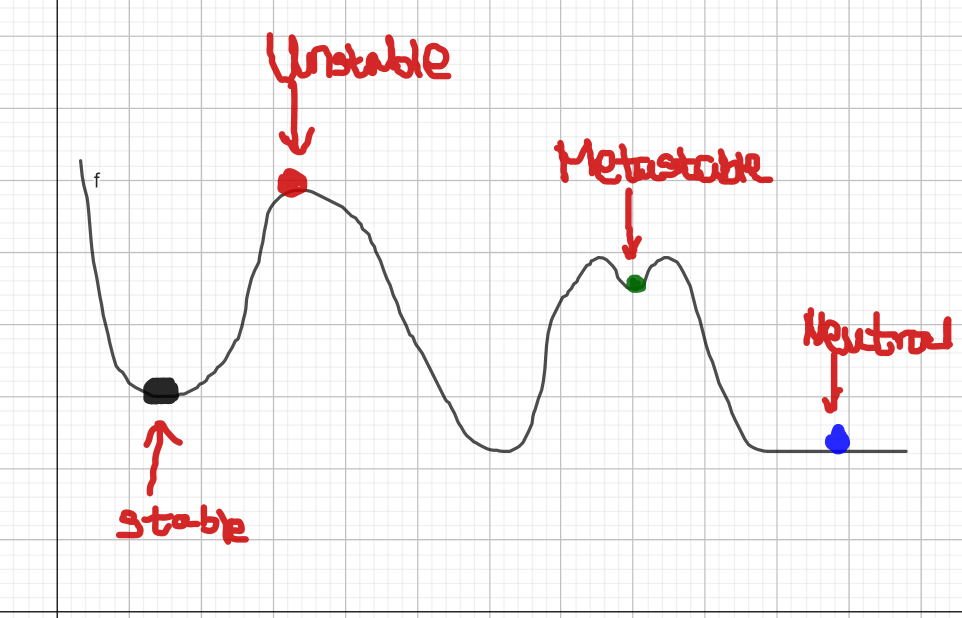
\includegraphics[scale=0.3]{resize_eqb.png}
    	\centering
    	\caption{Types of Equilibrium}
    	
    \end{figure}
    Examples of equilibrum:
   \begin{itemize}
   	\item A piston containing water vapour. Once this system reaches equilibrium it will be stable equilibrium. 
   	
   	\item A piston containing liquid water and water vapour. This system is in neutral equilibrium as upon compressing the piston the proportion of vapour and liquid will change but even at this new composition an equilibroum will be formed. Hence the system is in neutral equilibrium.
   	
   	\item A mixture of $H_2$ \& $O_2$ gas. If this system is compressed rapidly a combustion reaction will take place leaving us with water and heat(exothermic) because the mixture is reactive. However for small displacements the situation will be identical to that of stable equilibrium with water vapour. This is metastable equilibrium.
   \end{itemize}
    
    If a system undergoes no change when isolated from it's surroundings then it is said to be in thermodynamic equilibrium. For thermodynamic equilibrium the system needs to be in equilibrum with respect to all other potentials such as mechanical(force and torque balance), chemical(rates of reaction should be equal) and thermal.
    \pagebreak
\section{Zeroth Law}
    For two systems to remain in equilibrium the states of the system must remain constant. So atleast two of the independent thermodynamic variables must be constant. Two boundaries can exist such that there is equilibrium between two systems (i)diathermal and (ii)adiabatic. Diathermal boundary allows heat to be exchanged but not mass. 
    
    \begin{figure}[h]
    	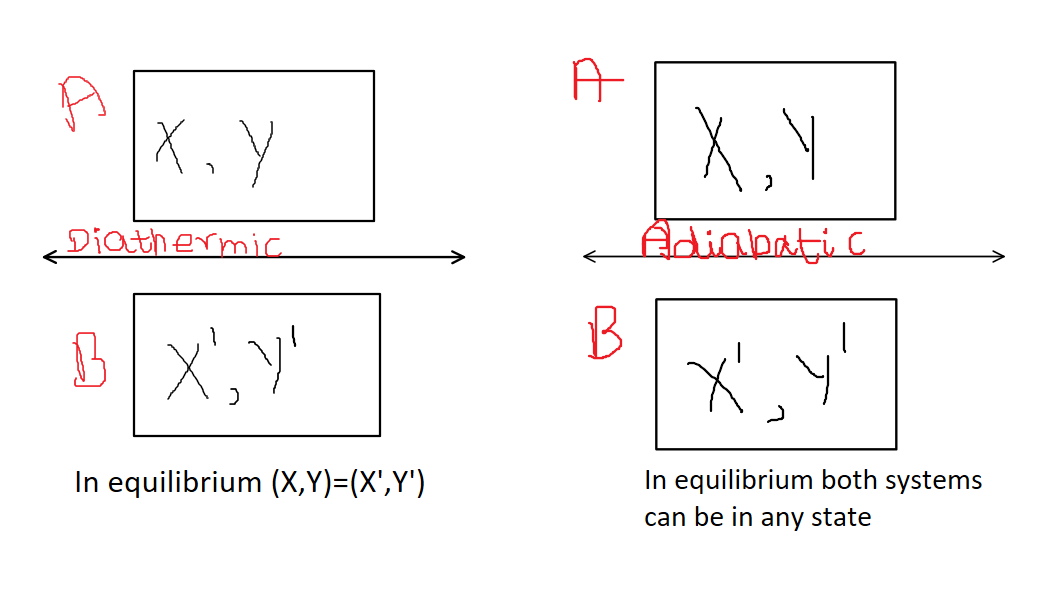
\includegraphics[scale=0.5]{zeroth_law.png}
    	\centering
    	\caption{Equilibrium with diathermic and adiabatic walls}
    \end{figure}
    \begin{tcolorbox}[title=Zeroth law]
    	IF there are three systems A, B, and C. 
    	\begin{itemize}
    		\item system A is in thermal equilibrium with system C
    		\item system B is in thermal equilibrium with system C
    	\end{itemize}
    then system A and B are in equilibrium.
    
    \end{tcolorbox}
   The idea of temperature developed after the idea of thermal equilibrium. If two systems are in thermal equilibrium then temperature is the common quantity which is constant for the two systems. Temperature is a scalar quantity. A necessary and sufficient condition for a system to be in thermal equilibrium is that its temperature is constant. If two containers are joined by a pipe with a two sided piston(2 plates joined by a rod) then we would say that the pressure in both containers is equal if the piston did not move. So the pressure was constant. Similarly in case of thermal equilibrium the temperature is constant. \\
   
   Consider the five isotherms below. The horizontal line cuts the isotherms at various X values. So we can say that the temperature along this line is a function of the X variable for a constant Y.
   \begin{figure}[h]
   	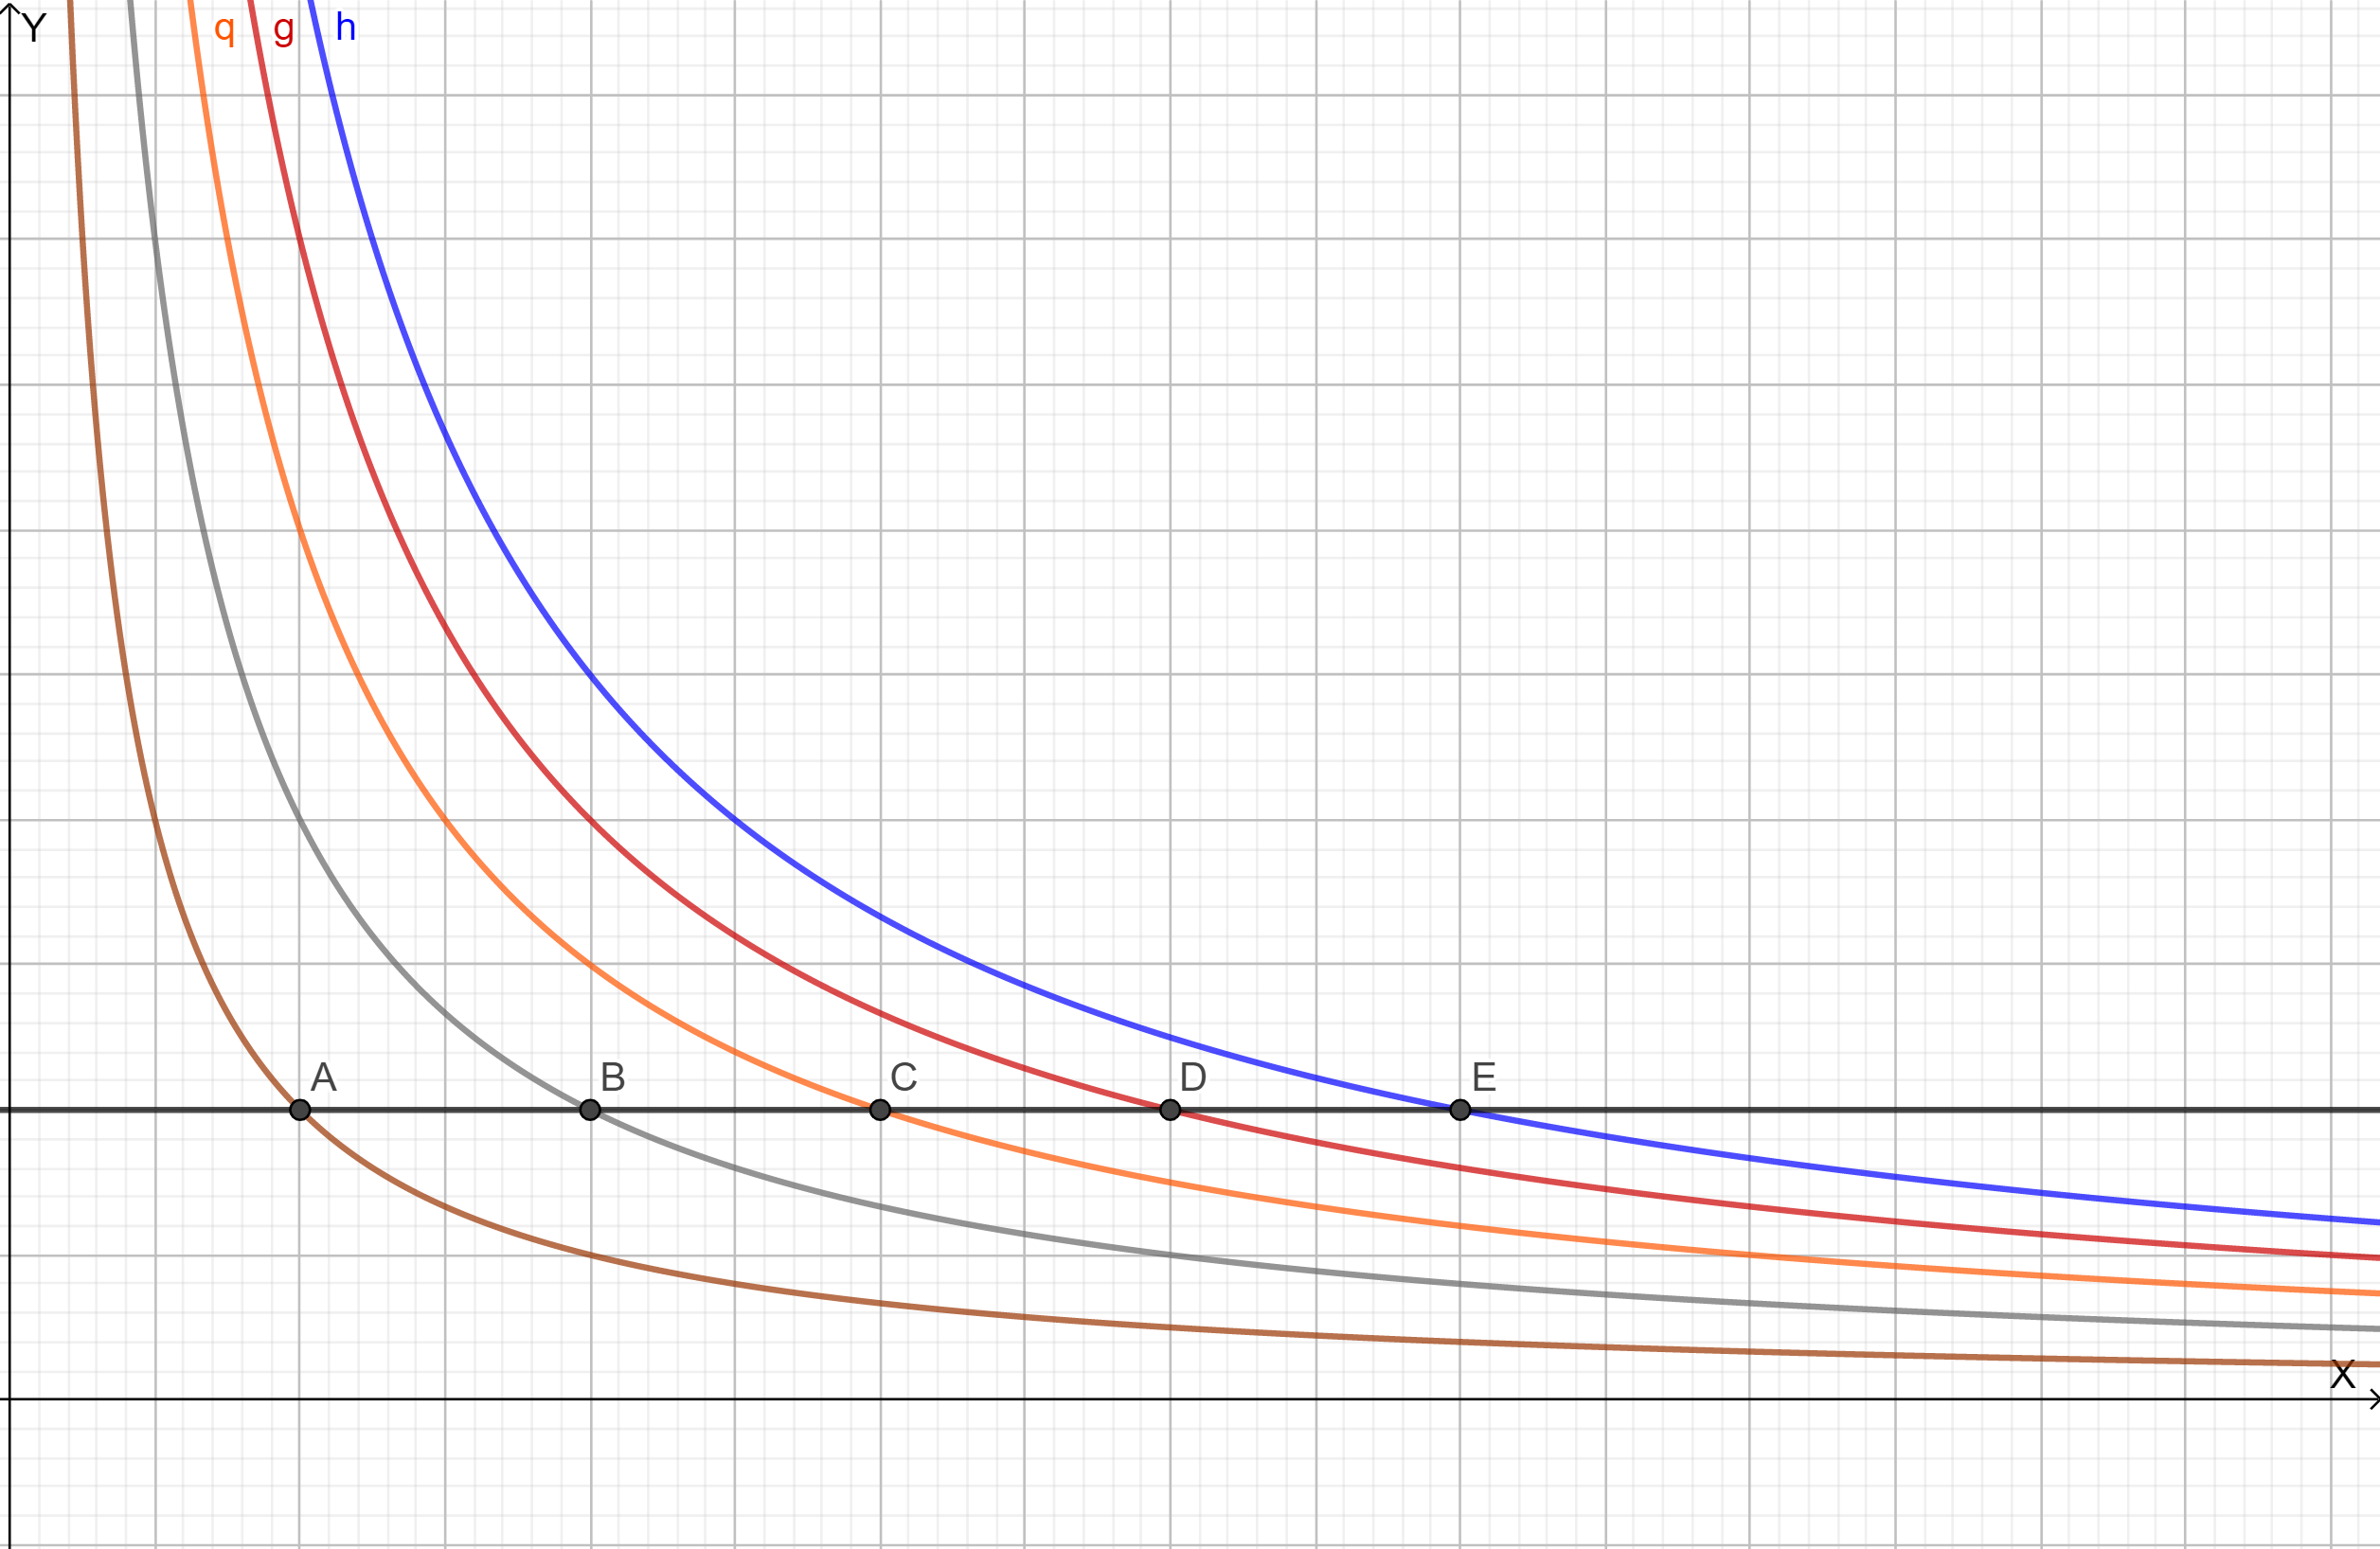
\includegraphics[scale=1.3]{thermometric.png}
   	\centering
   	\caption{Thermometric property}
   \end{figure}
    
    Let the temperature along the horizontal line be $\theta(X)$. We can linearly interpolate the temperature and get a relation for $\theta(X)$ as
    \begin{equation}
    	\theta(X)=aX \qq{for a fixed y}
    \end{equation}
    Here $X$ is the thermometric property for an inavriant $Y$. The first thermometer was a constant volume gas thermometer which means that $Y=V$ and $X=P$, it was an air thermometer developed by Santorio Santorio in 1612. \\
    
    To determine $a$ we must decide a fixed point which must be reproducible so that in any part of the world the same reference can be take. For the Celsius scale we take 2 reference point i.e. the temperature of ice-air saturated water equilibrium and of steam-water equilibrium. Air saturated water means water with 100\% humidity. The difference between the two fixed points is 100 degrees Celsius. This system is very difficult to reproduce as the equilibrium of ice with air saturated water is difficult to reproduce because ice is surrounded by water molecules. \\
    
    So an alternate definition is using a single point, the triple point of water(273.16 K) as a reference. So in order to find "$a$" 
    \begin{equation}
    	a=\dfrac{273.16}{\qq{Value of thermometric property X at 273.16 K}}
    \end{equation}
    Therefore the formula for temperature using a constant volume gas thermometer would be
    \begin{equation*}
    	\theta(P)=\frac{273.16}{P_{TP}}P
    \end{equation*}
    
    The basis for this scale is the ideal gas law(PV=nRT).
    
    \pagebreak
\section{Thermodynamic Systems}
    \subsection{Hydrostatic system}
    Any isotropic system of constant mass and composition that exerts on the surroundings a uniform hydrostatic pressure in the absence of gravitational, electric and magnetic effects we call a hydrostatic system.\\
    
    Every thermodynamic system has an equation of state. A hydrostatic system can be described by P, V and T as the thermodynamic variables. Plasma is also a fluid but it is a fluid consisting of ionic gases so electric and magnetic effects are also present hence it is not a hydrostatic system, therefore it's equation of state is more complicated and involves other variables. 
    
    \subsection{Work}
    If as system as a whole produces a change in it's surroundings and a displacement takes place, the work that is done either by the system or on the system is called external work. For hydrostatic systems
    \begin{equation}
    	dW=-P\underbrace{dV}_\text{compression} \qq{work done on the system is positive} 	
    \end{equation}

    In a finite quasistatic process the work done in going from volume $V_1$ to $V_2$ is
    \begin{align}
    	\int_{1}^{2} dW&=-\int_{V_1}^{V_2} PdV \\
    	       &=-\int_{V_1}^{V_2}P(T,V)dV
    \end{align}
    
    Since the process is reversible $W_{1\to2}=-W_{2\to1}$ provided they go along the same path. If the the process is cyclic then the net work done is given by $W=W_{1\to2}+W_{2\to1}$.
    \begin{equation}
    	W_{net}=\oint PdV 
    \end{equation}
    In a clock-wise cyclic process the net work done is negative and vice versa. In a CW process the work done is by the system as the magnitude of work done(area under the curve) in expansion is more than in compression hence the sum is negative. In an ACW process the reverse is true and the work done is positive.
    \subsubsection{Isothermal expansion of a gas}
   \begin{align}
   	W&=-\int_{V_1}^{V_2}PdV \\
   	 &=-nRT\ln(\frac{V_2}{V_1}) \\
   	 &=-nRT\ln(\frac{P_1}{P_2}) \qq{since $P_1 V_1=P_2 V_2$}
   \end{align}
   
   \subsubsection{Isothermal expansion for a solid}
   \begin{align}
   	dV&=\Bigg(\pdv{V}{P}\Bigg)_TdP+\underbrace{\Bigg(\pdv{V}{P}\Bigg)_PdT}_\text{=0 since isothermal} \\
   	  &=\Bigg(\pdv{V}{P}\Bigg)_TdP ,\quad \qq{$\kappa=-\frac{1}{V}\Bigg(\pdv{V}{P}\Bigg)_T$ is the isothermal compressibility}
   	\end{align}
   Therefore the work done in isothermal expansion of a solid is,
   \begin{equation}
   	W=\int_{P_1}^{P_2}\kappa PVdP \label{19}
   \end{equation}
   For systems where the volume does not change significantly, volume can be assumed constant and taken out of the integral in \eqref{19}.
   The formula for work done varies depending on the independent variables that define the system. Below is a summary of some of the common types of systems and the method to calculate the work done on them.
   \begin{center}
   	\begin{tabular}{|c | c | c |c |} 
   		\hline
   		System & Generalised force & Generalised disp. & Work Done  \\ [0.5ex] 
   		\hline\hline
   		Hydrostatic System & Pressure(P) in Pa & Volume(V) in $m^3$ & $-PdV$ \\ 
   		\hline
   		String & Tension(T) in N & Length(L) in m & $TdL$\\
   		\hline
   		Surface & Surface Tension($\gamma$) in N/m & Area(A) in $m^2$ & $\gamma dA$ \\
   		\hline
   		Electrochemical Cell & e.m.f($\mathcal{E}$) & Charge($\mathcal{Q}$) in C & $\mathcal{E}$d$\mathcal{Q}$ \\ [1ex]
   		\hline
   	\end{tabular}
   \end{center}
Since work done is path dependent it is an inexact differential and a differential amount is denoted by $\delta W$.

\subsection{Energy}
It is defined as the capacity to do work. Macroscopic forms of energy are kinetic and potential. These are called "organised forms of energy" because they can be readily converted to work. Microscopic modes of energy refer to the molecular and atomic structure of the system. \\

When a closed system completely surrounded by am adiabatic boundary is coupled with the surroundings such that work can be done, the work is called \textbf{Adiabatic Work}. Joule's experiment showed that the adiabatic work is not dependent on the path and depends only on the initial and final state of the closed system. This allows us to frame a restricted form of the first law of thermodynamics. 
\begin{center}
	\textit{"If a closed system is caused to change from an initial state to a final state by adiabatic means only, then the work done on the system is the same for all adiabatic paths connecting the two states"}.
\end{center}

So in case of adiabtic work we define a potential and an associated potential energy. Moving a charge in an electric field is an example of adiabtic work and there is an associated electric potential. The potential function associated is the internal energy(U). 
\begin{equation}
	W_{i-f}^{\text{Adiabatic}}=U_f-U_i
\end{equation}
If work is done on the system then $U_f>U_i$ and vice versa. Internal energy(U) is a state function hence it must be a perfect differential for e.g. in case of a hydrodynamic system $U=f(T,V)$. We mostly speak about the changes in internal energy as opposed to it's exact value. 
\begin{equation}
	dU=\Big(\pdv{f}{V}\Big)_TdV+\Big(\pdv{f}{T}\Big)_VdT
\end{equation}

\subsection{Molecular interpretation of internal energy}
Molecules have motional degrees of freedom such as translational, rotational and vibrational. The internal energy at 0K is due to the internal structure of the atoms. 
\begin{equation*}
U_m=U_m(0)+\tfrac{3}{2}kT
\end{equation*}
This is for a monoatmic substance which has only 3 DoF. Internal energy takes into account the kinetic energy of molecules and the potential energy due to interaction between atoms. Microscopic forms of energy relate to the structure and degree of molecular activity, this includes sensible(motional), latent, chemical and atomic. When the composition, structure and amount of a substance is fixed then the internal energy is determined only by temperature i.e. $U=f(T)$. \\

When work is done on a system with a diathermic boundary the work done is not entirely converted to internal energy and some energy is transferred as heat.  
\begin{center}
	"{\color{blue}When a closed system whose surroundings are at a different temperature and on which the diathermic work may be done, then energy transferred by non-mechanical means is called heat.}"
\end{center}

\section{First Law of Thermodynamics}

So if a system does work $w$ then it's internal energy decreases by $w$ and if it absorbs heat $q$ then it's internal energy increases by $q$. From here we get the FLOT,
\begin{tcolorbox}[title=First Law of thermodynamics(FLOT)]
	$$dU=\delta q-\delta w$$
Here $w$ is work done by the system. So in case of a gas it is $\int PdV$.
\end{tcolorbox}
\subsection{Constant-volume process}
 Work done in such a process is zero therefore, 
 \begin{equation}
 	dU=\delta q_v.
 \end{equation}

\subsection{Constant-pressure process(Enthalpy)}
Here the work nor the heat is zero therefore,
\begin{align*}
	                       dU&=\delta q_p-\delta w \qq{integrating,}\\
	                  U_2-U_1&=q_p-P(V_2-V1) \\
	                      q_p&=(U_2+PV_2)-(U_1+PV_1) \qq{so we define a new quantity H(enthalpy)}\\
	                        H&=U+PV\\
\end{align*}
There fore 
\begin{equation}
	\delta q_p=dH
\end{equation}
Now we can represent $U$ as $f(P,V)$ and get,
\begin{align*}
	dH&=dU+PdV+VdP \\
      &=\Bigg[V+\Bigg(\pdv{f}{P}\Bigg)_V\Bigg]dP+\Bigg[P+\Bigg(\pdv{f}{V}\Bigg)_P\Bigg]dV	
\end{align*}
Now if $H$ is an exact differential then it will be state function. We can see from above the $dH$ is in closed form hence enthalpy is a state function. In case of an ideal gas the internal energy is a function of temperature so at constant temperature the change in internal energy is zero. Now if we differentiate enthalpy with respect to pressure at constant temperature we get that the change in pressure is zero. So we conclude that enthalpy is constant with respect to pressure at constant temperature. Enthalpy is also only a function of temperature. 

Consider the following reaction
\begin{center}
	\ce{CaCO3 -> CaO + CO2}
\end{center}
Here the \ce{CO2} is formed as a gas hence the system expands and does work equal to $\int PdV$. So if we were to calculate the heat required to cause this reaction to occur then 
\begin{align*}
	q&=\Delta U+\int PdV\\
\end{align*}
In case of constant volume the heat of reaction/enthalpy will be equal to the internal energy change but in the constant pressure case the enthalpy will be different.The same is not true for the dissociation of calcium silicate where silica is formed in the solid phase. This is the significance of enthalpy.

\subsection{Heat Capacity}
This is a misnomer because they system does not hold heat but actually holds internal energy. It is not necessary that the temperature of a system should rise after inserting heat. In the case that it does we define the heat capacity as,
\begin{equation}
	C=\dv{Q}{T}.
\end{equation}
This heat capacity is an extensive property but we define the molar heat capacity which is intensive. The units of heat capacity is $JK^{-1}$. When there is no change in temperature such as when there is a phase change then the heat capacity would come out to be finite. The heat capacity will be different with respect to different independent variables of the system. For example in ideal gases we can have heat capacity at constant volume and at constant pressure.
For a hydrostatic system,
\begin{align}
	C_v&=\Bigg(\dv{Q}{T}\Bigg)_V \\
	C_p&=\Bigg(\dv{Q}{T}\Bigg)_P=\Bigg(\pdv{H}{T}\Bigg)_P
\end{align}
This can be extended for the independent variables of any system, for example for a wire the tension and length are independent variables, similarly for surfaces the area and surface tension are independent variables. If we consider the internal energy($U$) to be a function of T and V then we can get the following equation,
\begin{align}
	    \color{red}{dU}&\color{red}={\Bigg(\pdv{U}{T}\Bigg)_VdT+\Bigg(\pdv{U}{V}\Bigg)_TdV} \qq{worth remembering}\\
	          \dv{Q}{T}&=\Bigg(\pdv{U}{T}\Bigg)_V+\Bigg[\Bigg(\pdv{U}{V}\Bigg)_T+P\Bigg]\dv{V}{T}\\
\implies	        C_v&=\Bigg(\pdv{U}{T}\Bigg)_V
\end{align}
$C_p>C_v$ as $C_p$ includes the work done against pressure as well. We get the relationship between
the two as follows
\begin{align*}
                        C_p-C_v&=\Bigg(\pdv{H}{T}\Bigg)_P-\Bigg(\pdv{U}{T}\Bigg)_V\\
                               &=\Bigg(\pdv{(U+PV)}{T}\Bigg)_P-\Bigg(\pdv{U}{T}\Bigg)_V\\
                               &=\Bigg(\pdv{U}{T}\Bigg)_P+P\Bigg(\pdv{V}{T}\Bigg)_P-\Bigg(\pdv{U}{T}\Bigg)_V\\                        
                             dU&=\Bigg(\pdv{U}{T}\Bigg)_VdT+\Bigg(\pdv{U}{V}\Bigg)_TdV \\
\implies\Bigg(\dv{U}{T}\Bigg)_P&=\Bigg(\pdv{U}{T}\Bigg)_V+\Bigg(\pdv{U}{V}\Bigg)_T\Bigg(\pdv{U}{T}\Bigg)_P\\
\implies                C_p-C_v&=\Bigg(\pdv{V}{T}\Bigg)_P\Bigg[\Bigg(\pdv{U}{V}\Bigg)_T+P\Bigg]
\end{align*}
Here the term $\pdv{U}{V}_T$ is called the internal pressure of the system and is denoted by $\pi_T$. In case of ideal gases the internal pressure is $\pi_T=0$. So in case of ideal gases, $C_p-C_v=R$. When repulsive forces are dominant then $\pi_T<0$ and vice versa. For real gases one of the two cases is true.

\section{Joule-Thompson effect(throttling process)}
The adiabatic expansion of an ideal gas can be done in many ways. The temperature change experienced depends on the type of process. The first way is by a reversible prcoess which is isentropic, second way is free expansion into a vacuum. In the second case the work done will be zero hence in an adiabatic system the temperature change will also be zero. This is not true for perfect gases. The third way is the subject of the Joule-Thompson effect in which the gas moves from a pressure $P_1\to P_2$ with no change in kinetic energy(temperature is a representative of the kinetic energy). The third mechanism is \textit{isenthalpic}. The change in temperature of the gas with the pressure is called the Joule-Thompson ceofficient
\begin{equation}
	\mu_{JT}=\Bigg(\pdv{T}{P}\Bigg)_H=\frac{V}{C_p}(\alpha T-1). \label{30}
\end{equation} 
Here $\alpha$ is the coefficient of thermal expansion. All real gases have an inversion point at which the value of $\mu_{JT}$ changes sign. The temperature of this point, the Joule–Thomson inversion temperature, depends on the pressure of the gas before expansion. The expression \eqref{30} can be derived from
\begin{align}
                &	  \underbrace{\Big(\pdv{T}{P}\Big)_H}_{\mu_{JT}} \underbrace{\Big(\pdv{H}{T}\Big)_P}_{C_p} \underbrace{\Big(\pdv{P}{H}\Big)_T}_{1/\mu_{T}}=-1\\
              dH&=TdS+VdP
\end{align} 
where the $\mu_{T}$ is called the isothermal Joule-Thompson coefficient. 

\section{Thermochemistry}

Deals with the heat exchanges in chemical reactions and physical changes. 
\begin{align}
	dH=C_pdT && dU=C_vdT\\
\Delta H=H(T_2,P)-H(T_1,P) && \Delta U=U(T_2)-U(T_1)\\
        =\int_{T_1}^{T_2}C_pdT && =\int_{T_1}^{T_2}C_vdT
\end{align}

\subsection{Variation of $C_p \ \& \ C_v$}
Dulong and Petit found that all solids at room temperature have $C_v=3R=24.9 J/K$.The specific heats of compounds can be estimated using \textit{Kopp's rule} which says that the specific heat capacity of a solution is given by the weighted sum of the specific heats of it's components. If a compound is of the form \ce{A_xB_y} then it's heat capacity at constant volume is given by $x(C_v)_A+y(C_v)_B$.\\

$C_p$ is measured rather than $C_v$ as a more general expression can be obtained. The variation of $C_p$ with temperature(for all substances) can be fitted to the curve 
\begin{equation}
	C_p=a+bT+\frac{c}{T^2} \label{36}
\end{equation}
but only over a specific range of temperatures. For substances that exhibit polymorphism there can be abrupt changes in $C_p$ at the phase tranformation temperature and so the temperature change has to be specified.

\subsection{Variation of enthalpy with temperature}
If we have a reaction \ce{A + B -> C}, $\Delta H=q$ and if $q<0$ then the reaction is exothermic and if $q>0$ then it is endothermic. Enthalpy changes are reported under a set of standard conditions chief of which is that all components of the system initially and finally are in their respective standard states. Standard state of a substance(at a given temperature) is its pure form at 1 bar pressure. The enthalpy change for a physical or chemical process is the difference in the enthalpies of the products and reactants all at the same temperature and in their standard state.\\

Enthalpy can be changed by a change in composition or temperature and if it happens due to the latter then it is called sensible heat. These enthalpy change can be classified into four categories

	\subsubsection{Heat of reaction} 
	Enthalpy change when a chemical reaction takes place and by convention is assumed to be an isothermal process. Since enthalpy is a state function it is also independent of the path. Consider the reaction  
	\begin{center}
	\ce{A(pure) + BC -> AB + C}. 
	\end{center}
	For this the enthalpy change is given by 
	\begin{equation}
		\Delta H=\Delta H_{AB}+\Delta H_C-(\Delta H_A+\Delta H_{BC})
	\end{equation}
    However, if the process is not reversible then the temperature may change during the experiment though the intial and final temperatures will be the same. 
    \paragraph{Hess's Law of Constant Heat Summation}
    Since enthalpy is a state function. the change in enthalpy is also a state function. 
    \begin{center}
    	{\color{blue}"The total heat exchanged in a chemical process is the same irrespective of whether the process occurs in a direct single stage or through multiple stages"}
    \end{center}
    
    \paragraph{Kirchoff's Law}
    Used to calculate the $\Delta H$ at a different temperature than the one it is know at. If for a reaction performed at temperature $T_1$ the enthalpy change is $\Delta H_1$ and we want to find the enthalpy change $\Delta H_2$ at temperature $T_2$ then we can process by multiple paths. Firstly, perform the reaction at $T_1$ and then raise the products to $T_2$ 
    or perform the reaction itself at $T_2$. 
\begin{align}
    	\Delta H_b&=\Delta H_1 +\int_{T_1}^{T_2}C_p(\text{Products})dT \label{38}\\
    	\Delta H_a&=\Delta H_2 + \int_{T_1}^{T_2}C_P(\text{Reactants})dT \label{39} \\
 \text{Since}&\implies  \eqref{38}=\eqref{39} \\
\end{align}
\begin{equation}
	\boxed {\Delta H_2=\Delta H_1 + \int_{T_1}^{T_2}\Delta C_pdT}  
\end{equation}
  So we can also get the expression $$\Delta H_2-\Delta H_1=\int \Delta C_pdT$$ which can be written as the rate of change in heat of reaction with temperature,
  \begin{equation}
  	\boxed{\Bigg(\pdv{(\Delta H)}{T}\Bigg)_P=\Delta C_p}
  \end{equation}
Enthalpy of substances in their standard states at 1 atm pressure is assigned a value of zero. Whenever we express composition of gases we express it in volume fractions and all condensed phases are implied to be weight percentage. Flow metres for measuring flow of reactants into the chamber are calibrated to volume at 273K and 1 atm pressure. In case of an adiabatic process the intial enthalpy will be equal to the final enthalpy under isobaric condition




	 \subsubsection{Enthalpy change without aggregation} 
	 This means that the temperature of a substance is changed but no compositional change takes place i.e. \ce{A(298) -> A(T)}. So as a standard the enthalpy change is defined with respect to enthalpy at 298K. 
	$$\Delta H=\int_{298K}^{T}C_pdT$$ where $C_p$ is given by \eqref{36}.
	
	\subsubsection{Enthalpy change with aggregation} 
	Isothermal reactions but with compositional changes. Example, \ce{A(s) -> A(l)} at same the melting point $T_m$. 
	\subsubsection{Heat of mixing}
	If components are mixed to form a solution then $$\Delta H_{\qq{mixing}}=H_{\qq{solution}}-\sum H_{\qq{pure}} $$


\begin{tcolorbox}[title=Example]
	If we have reaction \ce{A_{(s)}(298 K) -> A_{(l)}(T_mK) -> A_{g}(TK)} then the enthalpy change is?
	\tcblower
    \begin{equation}
    	\Delta H=\int_{298}^{T_m}C_p dT + \Delta H_m +\int_{T_m}^{T_b} C_p dT + \Delta H_b + \int_{T_b}^{T} C_p dT
    \end{equation}
\end{tcolorbox}

\section{Adiabatic Flame Temperature}
Maximum temperature of the flame that can be achieved when some combustible fuel is burnt. Temperature will be maximum when conditions are adiabatic so that all the heat released is done via the flame. We are given some fuel at an initial temperature $ T_{i} $ and we want to find the maximum possible temperature of the flame $ T_{f} $ at the end of the reaction.
\begin{figure}
	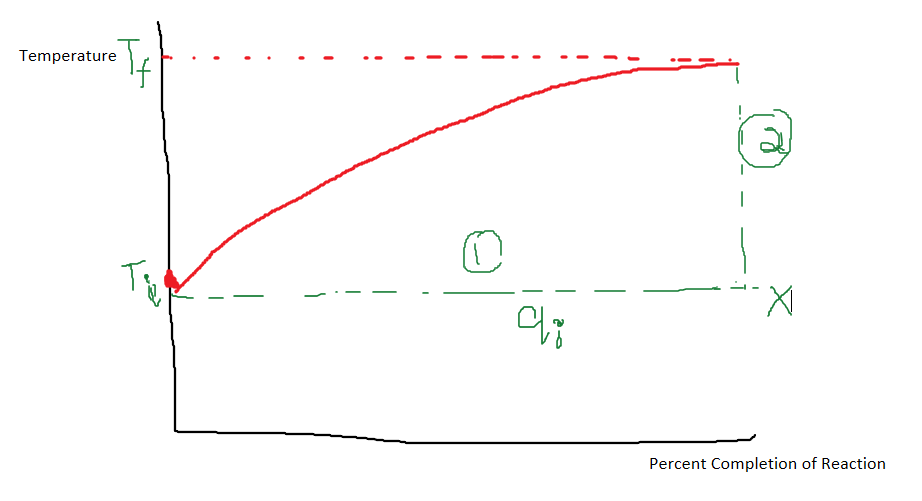
\includegraphics[scale=0.6]{adiabaticflame.png}
	\centering
\end{figure}
So the enthalpy change along path 1 is $\Delta H=H_X-H_i=-q_1$. The negative sign because heat is extracted out. The heat exchanged along path 2 will be equal but opposite because the whole process is negative. So we can say that, $$C_{\text{p,avg}}(T_f-T_x)=q_1 $$. Therefore 
\begin{equation}
	T_f-T_x=\dfrac{q_1}{C_{\text{p, avg}}} \label{45}
\end{equation}
if the initial temperature is known then the highest flame temperature for a theoretical 100\% completion can be found. In reality, few reactions go to 100\% completion due heat transfer, incomplete combustion, and dissociation. If we burn acetylene gas in insufficient oxygen then there will be soot formation i.e.e carbon monoxide will form which will cool and deposit carbon. If we use the stoichiometric amount of oxygen then we will have maximum adiabatic flame temperature. However, if the oxygen is in excess or air is used instead of oxygen then the flame temperature will be lowered because heat released from combustion will be absorbed by excess \ce{O2} or in case of air other gases like \ce{N2}. \\

For any adiabatic chemical process enthalpy and mass balance are valid(except nuclear). Mass balance is simply equating the mass on both sides. Since enthalpy is an extrinsic  property we have to multiply by number of moles. We can calculate the enthalpy at different temperatures using Kirchoff's law. $$\sum n_i H_{i}^{T_i}=\sum n_j H_{j}^{T_j} $$

In \eqref{45} the $ C_p $ should include all the components present in the chamber. This includes excess reactants and products as well. Normal cubic meter is measured at 0 degrees Celsius and standard cubic meter is measured at 15 degrees Celsius. 

\section{Applications of the first law}
\subsection{Isothermal Process}
$$ dT=0\ \& \ dU=0$$So we get
\begin{align*}
    dQ&=PdV\\
    dQ&=RT\ln(\frac{V_f}{V_i})\\
    dW&=-dQ
\end{align*}

\subsection{Adiabatic Process}
\begin{align*}
	dQ&=0\\
	dW&=dU\\
  -PdV&=nC_VdT	
\end{align*}
Substituting P=RT/V giving us the common relationships
\begin{align}
	    PV^\gamma&=\text{Constant}\\
	TV^{\gamma-1}&=\text{Constant} 
\end{align}
We can also calculate the enthalpy as follows 
\begin{align}
	           dH&=VdP\\
\implies \Delta H&=\dfrac{\gamma P_iV_i}{\gamma-1}\Bigg[\Bigg(\dfrac{V_i}{V_f}\Bigg)^{\gamma-1}-1\Bigg]
\end{align}

\subsection{Polytropic process}
\begin{equation}
	PV^n=\text{Constant}
\end{equation}

Work done in an isothermal is greater than in an adiabatic process because some of the work done in an isothermal process goes towards heat whereas for an adiabatic process the internal energy decreases at the expense of the work with no heat exchange. 

Questions left unanswered by the first law:
\begin{enumerate}
	\item What magnitudes may the q and w effects have?
	\item What criteria governs these magnitudes?
	\item Is there a limit to the amount of work which a system can do during it's change?
\end{enumerate}

\section{Second Law of Thermodynamics}
 Also called the "law of degradation of energy". Consider a cup with hot coffee in it, it is intuitive that the cup will cool with time. However we do not expect the cup to get hotter whilst cooling the surrounding. The energy converts from an organised form to a more disorganised form. If a system is left to itself it will do one of two things (i)remain in the same state or (ii)move of its own accord to some other state. The second process is termed  spontaneous because the process starts without external influence and moves towards equilibrium so there is a definite direction. All natural processes are spontaneous and irreversible.\\

\begin{center}
	{\color{red}"A process which involves the spontaneous movement of a system from non-equilibrium state to an equilibrium state is called a natural/spontaneous/real process".}
\end{center}
 
 \paragraph{So what determines the direction of spontaneous change?}
 The total energy of an isolated system is constant but isolated systems can also undergo spontaneous processes. The direction of change is determined by the distribution of energy. As a system undergoes a spontaneous process it's ability to do work reduces i.e. it's energy dissipates. All real processes are irreversible where energy dissipates and the amount that dissipates depends on the path followed. 

\section{Degree of Irreversibility}
Consider the conversion of mechanical work to thermal energy. Consider a reservoir maintained at constant temperature "T" with a paddle wheel inside which is rotated using energy from a falling weight by means of a pulley. If the pulley does "w" work and "q" heat gets transferred to the reservoir. If we take the reservoir to be at a lower temperature then the transfer of heat will be more irreversible. So the degree of irreversibility is proportional to the heat exchanged and inversely proportional to the temperature of the system. We assign the entropy change of a system that absorbs energy "q" at temperature "T" the value 
\begin{equation}
	\Delta S=\frac{Q}{T}
\end{equation}
Now if we consider infinite number of reservoirs(with imperceptible temperature change across each) connected to each other and the first one connected by a paddle wheel then the differential form is
$$dS=\frac{dQ}{T}$$
Let us now examine if entropy is a state function. First, write dQ in differential form as
\begin{align}
	dQ&=\Bigg[\Bigg(\pdv{U}{V}\Bigg)_T+P\Bigg]dT+\Bigg(\pdv{U}{T}\Bigg)_V dT\\
      &=\frac{RT}{V}dV+\Bigg(\pdv{U}{T}\Bigg)_V dT	\\
    \frac{dQ}{T}&=\frac{R}{V}dV+\frac{1}{T}\Bigg(\pdv{U}{T}\Bigg)_V dT\\
\end{align}
The above differential equation is in closed form hence dS is an exact differential i.e. entropy is a state function.

 \begin{figure}[h]
    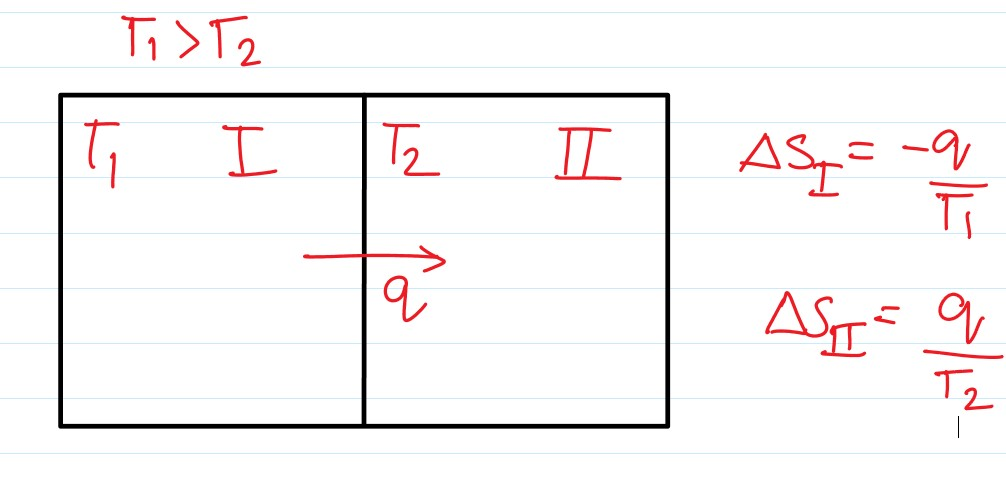
\includegraphics[scale=0.5]{signofentropy.jpg}
    \centering
 \end{figure}
In the above figure the net change in entropy for the irreversible process(when $T_1\neq T_2$) is given by 
\begin{equation*}
	\Delta S_{\text{irreversible}}=\dfrac{q(T_1-T_2)}{T_1 T_2}
\end{equation*}
For a reversible process to occur $T_1=T_2$ and in that case $\Delta S_{\text{reversible}}=0$. For $T_1>T_2$, 	$\Delta S_{\text{irreversible}}>0$ and vice versa. The values of q and w for a process are limited by the second law of thermodynamics i.e. a $q_{\text{max}}$ and $w_{\text{max}}$ for any system undergoing a process. Consider two processes (i)reversible isothermal expansion of an ideal gas and (ii)free expansion. \\

So for the first process the heat exchanged is equal to the work done as the internal energy is constant. 
\begin{align*}
	q_{\text{reversible}}&=RT\ln(\frac{V_A}{V_B})\\
	\Delta S_{\text{reversible}}&=R\ln(\frac{V_A}{V_B})\\
\end{align*}
Now as for the heat reservoir that maintains the temperature of the ideal gas the entropy change bears the opposite sign making the total entropy change of the system equal to zero. Now consider the case of free expansion where the process is irreversible. In free expansion the work done is zero and for an ideal gas the change in internal energy is also zero. This gives $q=0\implies \Delta S_{\text{reversible}}=0$. However the entropy of the gas obviously changes as it expands. Since entropy is a state function the entropy change will be same as that in reversible isothermal expansion provided the initial ad final states are the same. 
\begin{equation}
	\boxed{\Delta S_{\text{gas}}=\Delta S_{\text{gas in rev process}}=R\ln(\frac{V_B}{V_A})>0}
\end{equation}
\subsection{Maximum heat and work}
From the above analysis we can say that the most heat that can be transferred to the gas is in the case of a reversible isothermal expansion because all the work done is transferred as heat and none of it goes into changing the internal energy. Similarly the maximum work that can be done by gas is in the case of an isothermal reversible expansion for the same reason. 
\begin{align}
	0\leq w&\leq w_{\text{max}}\\
    0\leq q&\leq q_{\text{max}}
\end{align}
The minimum in both cases arises from free expansion. Similarly we can get bounds on the entropy change of a system as well. 
\begin{equation}
	\boxed{0\leq \Delta S_{\text{Total}}\leq \frac{q_{\text{rev}}}{T}}
\end{equation} 
Note that although the maximum entropy change is denoted by $q_{\text{rev}}$ it actually arises in the irreversible process however the magnitude of heat exchanged is the same as in case of a reversible process between the same two states. The minimum is in case of a reversible process. The magnitude of $q$ depends on the degree of irreversibility of the process. 
\begin{align}
	dS&=\frac{dQ_{\text{rev}}}{T}\\
    dQ&=C_pdT-VdP\\
    dS&=\frac{C_p}{T}dT-\frac{V}{T}dP\\
      &=\frac{C_p}{T}dT-nRdP\\
\end{align}
\begin{equation}
	\implies \boxed{\Delta S= \int_{T_i}^{T_f}C_p \frac{dT}{T}-\int_{P_i}^{P_f}nR \frac{dP}{P}}
\end{equation}
 Above calculation was done considering heat as a entropy as a function of temperature and pressure. If we consider it a function of volume and temperature then
 \begin{equation}
 	dS=C_v\frac{dT}{T}-nR\frac{dV}{V}.
 \end{equation}

Adiabatic process are isentropic because no heat is exchanged by the system. 
{\color{red}doubt about reversible and irreversible adiabatic expansion.}
\subsection{Entropy change for reversible(equilibrium) phase change}
\begin{align}
	\Delta S&=\int \frac{dQ}{T}\\
	        &=\frac{\Delta H}{T}
\end{align}
\subsection{Entropy change in mixing of ideal gases}
	Two ideal gases are mixed at constant temperature and pressure then their entropy change can be written as the sum of entropy changes of each gas. Entropy change of each gas can be written as
\begin{equation}
		\Delta S_A=n_AR\ln(\frac{V_A+V_B}{V_A}) 
\end{equation}
So the total entropy change can be written as follows where X denotes the mole fraction of the gas
\begin{equation}
	\Delta S=-R\Big[X_A\ln(X_A)+X_B\ln(X_B)\Big]
\end{equation}

\begin{figure}[h]
	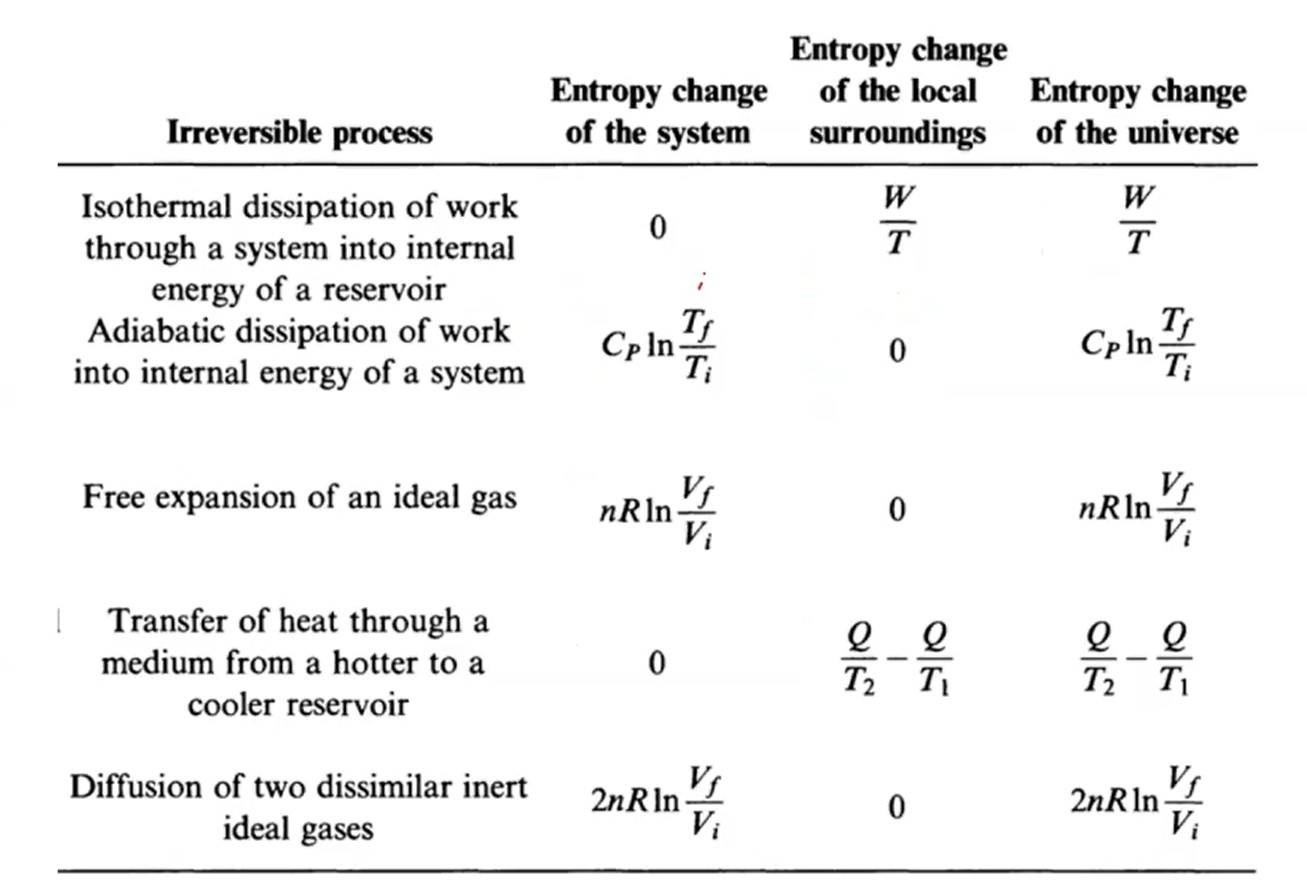
\includegraphics[scale=0.5]{tableofentropy.jpg}
	\centering
\end{figure}

\begin{tcolorbox}[title=Second Law of Thermodynamics]
	\begin{enumerate}
		\item Entropy is a thermodynamic state variable(function).
	    \item Entropy is not created when a system undergoes a reversible process: it is transferred from one part of the system/surroundings tp another part.
	    \item The total entropy of the universe increases when an irreversible process occurs.
	    \item For all processes, the entropy of the universe increases or stays the same. The total entropy of the universe never decreases. 
	\end{enumerate}
\end{tcolorbox}

\section{Caratheodary formulation of $2^{nd} law$}
This formulation does not involve cycles and heat engined and takes a mathematical approach to deriving the second law. A differential expression of the form 
\begin{equation}
	dL=\sum_i X_i dx_i \qq{is called a Pfaffian differential.}
\end{equation}

\begin{tcolorbox}[title=Caratheodary's Theorem]
	If a Pfaffian expression has the property for which, in the neighbourhood of any point P, there are points that cannot be connected to P along curves that satisfy the equation $dL=0$, then the Pfaffian expression has an integrating factor.
\end{tcolorbox}
So an inexact differential that follows the condition $dL=0$ can be made exact via an integrating factor. Caratheodary showed that $\delta q=\sum x_i dx_i$ can be made exact using an integrating factor. This means that \textit{in the neighbourhood of every equilibrium thermodynamic state, there exist states unattainable from it by any adiabatic process(reversible or irreversible)}. So a state function has a tendency to increase. \\

Reasoning behind Caratheodary's theorem:\\
\subsection{Existence of an integrating factor:}\label{caratheo1}
$$dU=\delta q+PdV$$ Let $U=f(T,V)$,
\begin{align*}
	 \delta q&=\Bigg[\underbrace{\Bigg(\pdv{U}{V}\Bigg)_T}_{=0}+P\Bigg]dV+\Bigg(\pdv{U}{T}\Bigg)_VdT \\
	 \delta q=\frac{RT}{V}dV+\Bigg(\pdv{U}{T}\Bigg)_VdT \\
\end{align*}
we can see that $\delta q$ is not an exact differential. Whereas, if we divide by T then the equation becomes exact. Hence for an ideal gas($\pdv{U}{V}$=0) $\frac{1}{T}$ is an integrating factor. 
\begin{align}
	\dfrac{\delta q}{T}&=\frac{R}{V}dV+\frac{1}{T}\Bigg(\pdv{U}{T}\Bigg)_VdT\\
	\dfrac{\delta q}{T}&=dS\\
	\implies \frac{1}{T}&\to \text{Integrating Factor}
\end{align}
Caratheodary showed that for complex systems as well $1/T$ is an integrating factor. Therefore $\frac{\delta q_\text{rev}}{T}$ is an exact differential or all systems.

\subsection{In the vicinity of an eqb. state there exist states unattainable by an adiabatic process} \label{Caratheo2}
Consider a system having two independent variables $\theta$ and $x_1$. By the Duhem postulate we can define the state of the system using these two variables. 

\begin{figure}[h]
	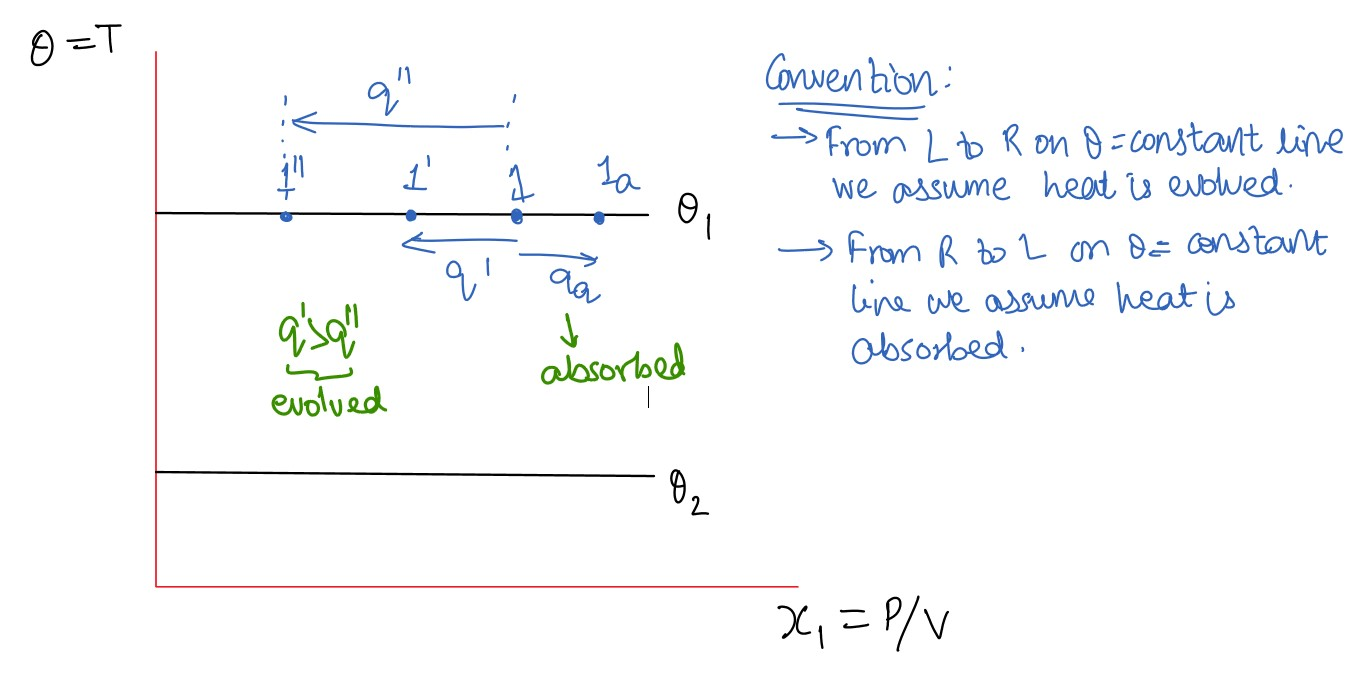
\includegraphics[scale=0.6]{caratheodary1.jpg}
	\centering
	
\end{figure}
We need to show that there are states unattainable from the state $\theta_1$ to $\theta_2$ by a reversible/irreversible adiabatic process. So consider the path $1\to 2'\to 1'\to 1$ as shown below. In this cycle heat is absorbed only along $1'\to 1$ as all other processes are reversible adiabatic. Since it is a cyclic process the internal energy change is zero therefore all the heat absorbed must be converted to work which is highly improbable. Similarly we can consider any path say for e.g. $1\to 2_a\to 1_a\to 1 $. Here the heat is evolved along $1_a\to 1$ and so all the work done is liberated as heat. This is not forbidden by the laws of thermodynamics. Therefore any point to the right of \textbf{1} are accessible by a reversible/irreversible \textbf{adiabatic} process. \\

\begin{figure}[h]
	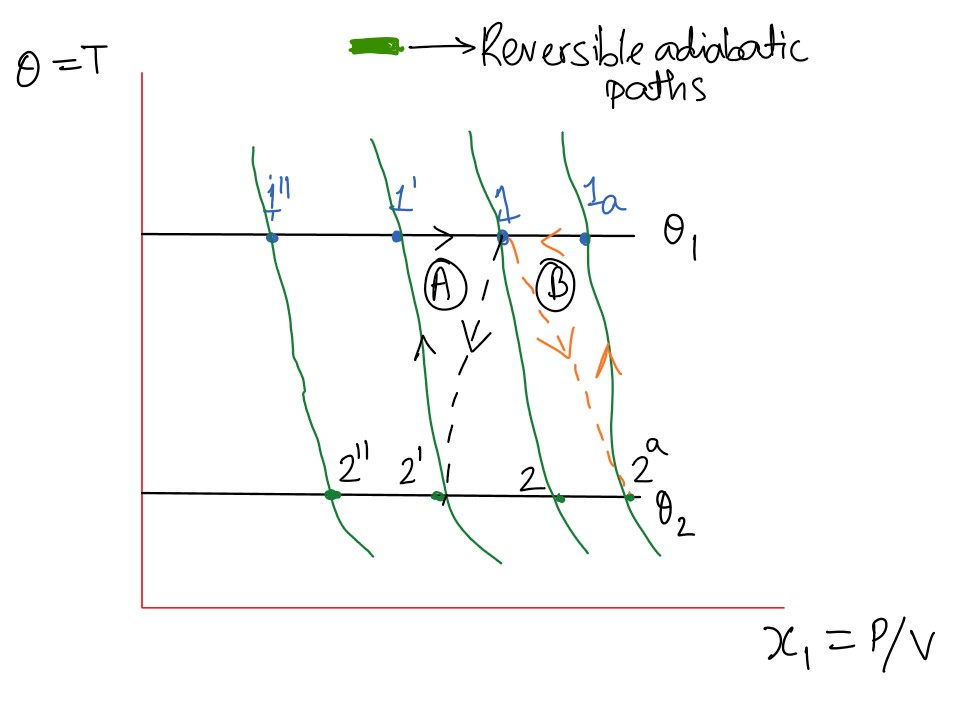
\includegraphics[scale=0.6]{caratheodary2..jpg}
	\centering
\end{figure}

We can still access points to the left of state \textbf{1} but not by an adiabatic process. We can go from $1\to 2_a$ by $1\to 1_a \to 2_a$ where the heat is absorbed hence the state function(entropy) is increasing since $dS=\int dQ/T$. If we consider the reverse process i.e. $2_a\to 1$ via $2_a\to 1_a\to 1$ then the heat will be evolved(consequence of the sign convention) making entropy change negative. It follows that the first process is feasible but the second isn't as \textbf{1} is to the left of $2_a$.

\subsection{State function must increase for a spontaneous adiabatic process and remain constant for a reversible one} \label{caratheo3}

This entire formulation is a consequence of $\delta q=\sum X_i dx_i$ being an exact differential upon dividing by $T$. Since $dS=0$ is an exact differential the integral curves will be of the form 
\begin{equation}
	S_k(x_1,x_2,\cdots x_n)=C_k, \qq{where $C_k$ is a constant with $k\in \{1, 2, 3,\cdots n\}$}
\end{equation} 
with each of the solutions being isentropic surfaces(entropy is a state function). There will therefore be no reversible adiabatic process that can allow a system to go from the surface $S_i$ to $S_j$ as that process won't be isentropic and hence not adiabatic reversible. However we can go between two isentropic states by an irreversible process however it will only be favourable for $i \to j$ such that $S_j>S_i$. Therefore our state function(entropy) must increase for a spontaneous adiabatic process, but remain constant for reversible adiabatic ones. So there is a natural or thermodynamic sense of direction for adiabatic processes. \\

Consider a series of heat reservoirs connected by diathermic walls and the entire set up with an adiabatic boundary. Heat will be transferred between the reservoirs such that the net entropy change is zero. 

\begin{figure}[h]
	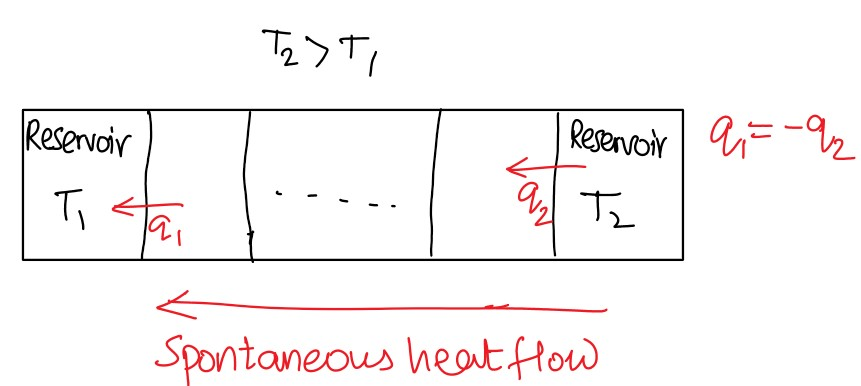
\includegraphics[scale=0.8]{caratheodary3.jpg}
	\centering
\end{figure}

So net change in entropy will be given by

\begin{align*}
	\Delta S_1&=\dfrac{q_1}{T_1}\\
	\Delta S_2&=\dfrac{q_2}{T_2}\\
	\Delta S_{net}&=q_1\Bigg(\dfrac{1}{T_1}-\dfrac{1}{T_2}\Bigg)\\
	\implies \Delta S_{\text{process}}&>0
\end{align*}
So if the entropy change is positive then the process will be spontaneous and natural. To summarise Caratheodary's formulation, 
\begin{enumerate}
	\item There are states around an equilibrium state to which adiabatic paths are not possible. How do we know this? From section \ref{Caratheo2}.
	\item In such cases an integrating factor exists for the Pfaffian expression. How do we know this? From section \ref{caratheo1}.
	\item The exact differential we get after multiplying by the integrating factor is $dS$ and its solution function has  a tendency to increase when undergoing an irreversible adiabatic process. How do we know this? From section \ref{caratheo1}, \ref{Caratheo2} and \ref{caratheo3}.
\end{enumerate}

\section{Heat Engines and Refrigerators}
\subsection{Conversion of work to heat}
Consider rubbing two stones, the work done in rubbing results in a rise in temperature of the stones. If this setup is underwater then the work done will be transferred to the water as heat and the temperature of the water will increase. Similarly if we place a resistor under water and a pass a current through it then in an ideal scenario the temperature of the water will rise with no change in the thermodynamic state of the resistor. Since there is no change in state of the thermodynamic system(stones or resistor) the change in internal energy is zero therefore $w=Q$. In the case of conversion of work to heat there is no change in the state of the system therefore the process can be repeated indefinitely.\\

Consider the isothermal expansion of an ideal gas. The work done by the gas is equal to the heat absorbed. However, in this case the state of the system changes as the gas expands and changing $P$ and $V$. Thus it cannot be done indefinitely. So if we want to do such a process indefinitely then we need to perform a series of steps. This concept is used in a heat engine. 

\subsubsection{Heat Engine}
\begin{figure}
	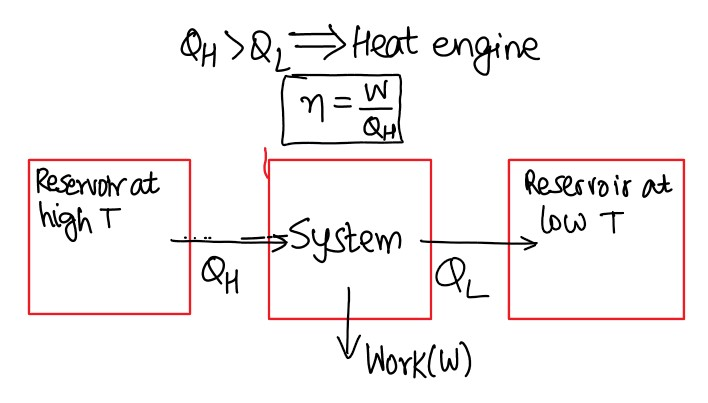
\includegraphics{heatengine.jpg}
	\centering
\end{figure}
The system receives heat $Q_H$ from a high temperature reservoir and rejects $Q_L$ heat to a lower temperature reservoir whilst doing work $W$ on it's surroundings. The efficiency of this process is given by
\begin{equation}
	\eta=\dfrac{\text{Work Done(W)}}{\text{Heat Input}(Q_H)}
\end{equation}
From FLOT, $$Q_H-Q_L=W.$$
No heat engine has been developed that converts all the heat extracted from a high temperature reservoir to work without rejecting any heat to a low temperature reservoir. 
The statements of Kelvin and Planck can be combined to give the combined Kelvin-Planck statement of the second law of thermodynamics.
\begin{tcolorbox}[title=Kelvin-Planck Statement of the Second Law]
	It is impossible to construct an engine that, operating in a cycle, will produce no effect other than the extraction of heat from a reservoir and the performance of an equivalent amount of work.
\end{tcolorbox}
The above statements also implies that a perpetual motion machine can never be made.

\subsubsection{Refrigeration Cycle}
\begin{figure}[h]
	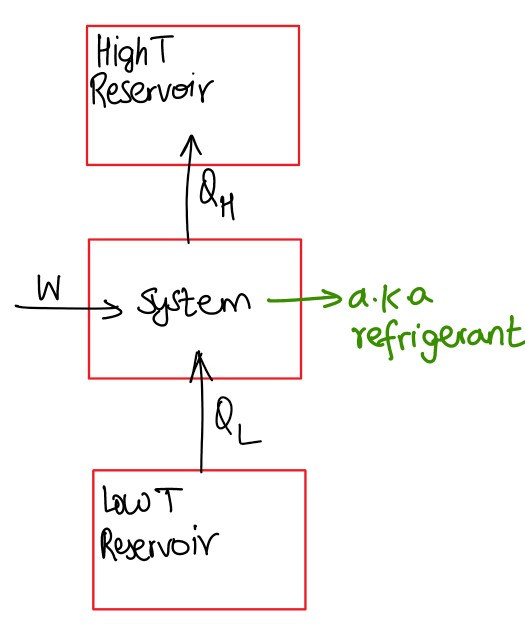
\includegraphics[scale=0.8]{refrigeration.jpg}
	\centering
\end{figure}
A machine that performs work in the opposite direction as a heat engine is called a refrigerator and the working substance(system) is called the refrigerant. The refrigerator takes in heat $Q_L$ from the low temperature reservoir after work $W$ is done on it, it rejects heat $Q_H$ to a high temperature reservoir. 
$$Q_H=W+Q_L$$
The work done is necessary to transfer the heat from the low temperature reservoir to a high temperature reservoir as it is not a spontaneous process. This gives us the Clausius statement of the second law.
\begin{tcolorbox}[title=Clausius Statement of the Second Law]
	It is impossible to construct a refrigerator that, operating in a cycle, will produce no effect other than the transfer of heat from a lower-temperature reservoir to a higher-temperature reservoir.
\end{tcolorbox}
Both statements for the second law are equivalent. We can prove this by showing that the negatives and positives of the statements are equivalent. 

\subsubsection{Carnot's Cycle}
\begin{tcolorbox}[title=Carnot's Theorem]
	No heat engine operating between two given reservoirs can be more efficient than a Carnot engine operating between the same two reservoirs.
    \tcblower
    Corollary: All Carnot engines operating between the same two reservoirs have the same efficiency.
\end{tcolorbox}
A Carnot cycle is a set of processes that can be performed by any thermodynamic system. Any engine performing a Carnot cycle is called a Carnot engine. The Carnot cycle has a system in thermal equilibrium with a reservoir at the low temperature T. This is advantageous as compared to the heat engine or refrigerator. The Carnot cycle has 4 processes, 2 adiabatic and 2 isothermal. Irrespective of the kind of system we choose, these 4 processes must be performed. 

\begin{figure}[h]
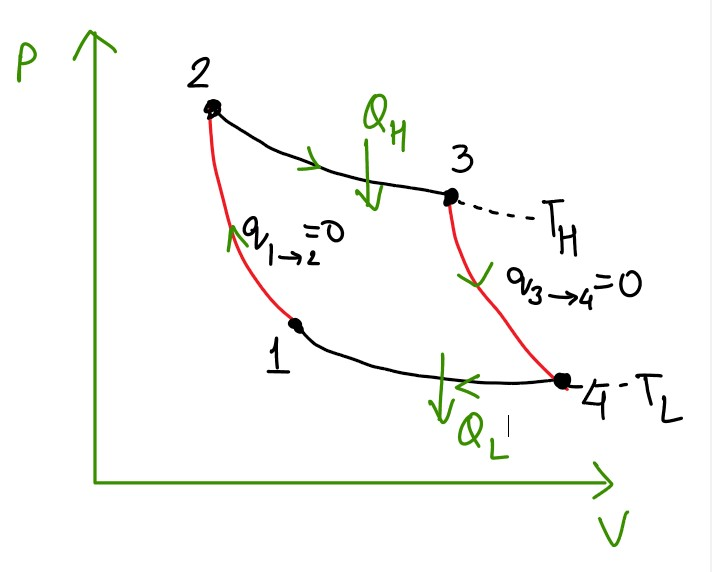
\includegraphics[scale=0.6]{carnot.jpg}
\centering
\end{figure}
The Carnot engine rejects $Q_L$ heat to the low temperature reservoir and absorbs $Q_H$ heat from the high temperature reservoir. If we reverse the path of the cycle i.e. if we reject heat to the high temperature reservoir and take up heat from the low temperature reservoir then we get Carnot's refrigeration cycle. The efficiency of the engine depends only on the reservoirs between which the engine operates and is completely independent of the working material. \\

The Carnot cycle is reversible, has only two reservoirs, absorbs heat at $T_H$ and rejects heat it at $T_L$ and its efficiency is independent of the system.
\begin{equation}
	\eta_R=1-\frac{Q_H}{Q_L}
\end{equation}
So we can say that the efficiency of the Carnot cycle is given as 
$$\eta=\frac{Q_1}{Q_2}=f(T_1,T_2)$$
it can be proved that 
\begin{equation}
	\eta_{\text{Carnot}}=1-\dfrac{Q_L}{Q_H}=1-\dfrac{T_L}{T_H}
\end{equation}
If we calculate the entropy change of the system used in the heat engine,
\begin{align*}
	\Delta S&=\frac{Q_H}{T_H}-\frac{Q_L}{T_L}\\
	\Delta S&=0.
\end{align*}
Therefore for an ideal heat engine the entropy change of the system is zero. Note also that cycle only consists of reversible reactions. 
\\

So the efficiency is the ratio of the absolute temperatures of the two reservoirs therefore the Carnot engine can be used to define the absolute temperature scale. We can set up the adiabatic conditions and measure the heat exchanged in the isothermal processes. The ratio of which will give the ratio of temperatures. Let us take the reference temperature of 273.16 K as the triple point of water($T_{TP}$). So if we set up a Carnot cycle between $T_{TP}$ and some unknown temperature T then the temperature $T$ can be determined as
\begin{equation}
	T=273.16\times \frac{Q_T}{Q_{TP}}K
\end{equation}
One can see that in this scale the heat exchanged by the reservoir in the isothermal process is the thermometric property. If the heat exchanged by the reservoir in a reversible process is zero then the reservoir is at absolute zero temperature. This goes to show that absolute zero is independent of the system. Therefore only when $T_L=0$ the efficiency will be 1. 

\section{Clausius's Inequality}
Consider the process $i \to f$ shown below. The path is isothermal and let's denote the work done by $W_{i\to f}$. Take two points a and b on adiabatic curves such that the work done in the process $i\to f$ is the same as that in $i\to a\to b\to f$. We see that,

\begin{figure}
	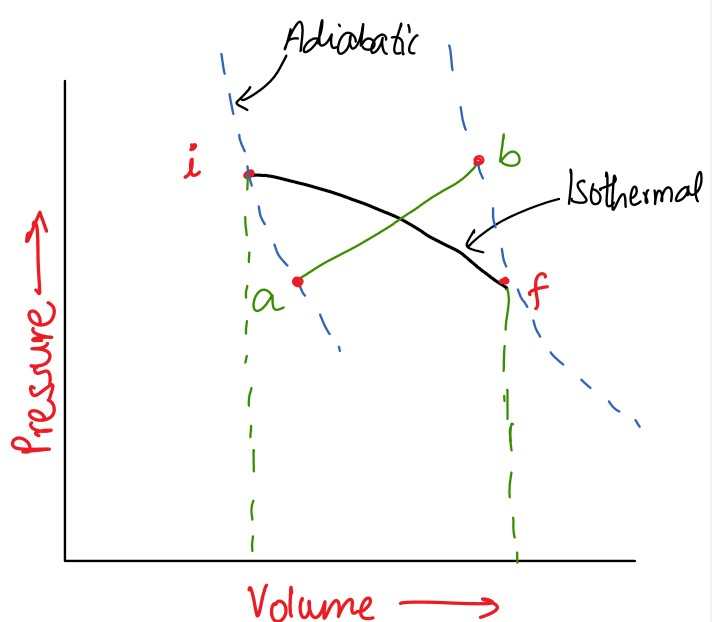
\includegraphics[scale=0.6]{clausius.jpg}
	\centering
\end{figure}

\begin{align*}
	W_{if}&=W_{iabf}\\
	Q_{if}&=Q_{iabf}=Q_{ab} \text{since i$\to$ a and b$\to$ f are adiabatic.}
\end{align*}
Now consider a cyclic process as shown below. 
\begin{figure}[h]
	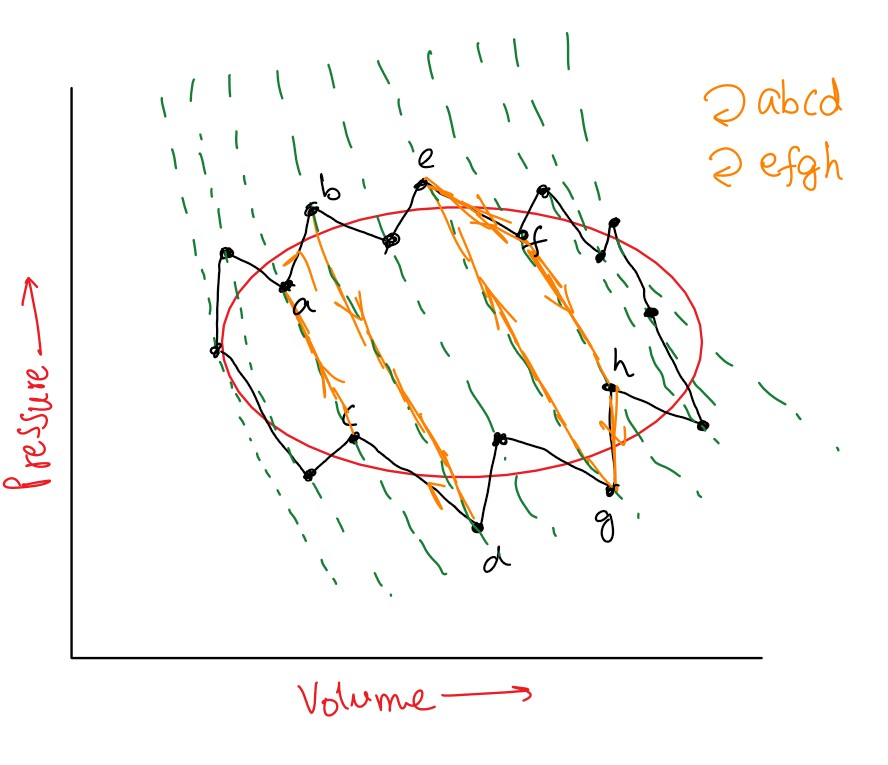
\includegraphics[scale=0.6]{clausius2.jpg}
	\centering
\end{figure}
Here in the process a$\to$ b the heat exchanged $Q_1$ is negative of that in process c $\to$ d. Between any two adjacent adiabatic curves we can find two such paths.The entire cyclic process can be described by the zig-zag path shown. So the total entropy over the entire cyclic process will be zero.
\begin{equation}
	\oint_R \dfrac{dQ}{T}=0
\end{equation}
This is the first part of the Clausius statement of the second law and concerns only reversible processes as all the zig-zag lines along with the adiabatic lines make up a Carnot cycle. For an irreversible process we get $$\oint_I \dfrac{dQ_I}{T}<0.$$
We can combine the two statements of Clausius into one inequality,
\begin{tcolorbox}[title=Clausius's Inequality]
	\begin{equation}
	\oint \dfrac{dQ}{T}\leq 0
	\end{equation} 
\end{tcolorbox}
Consider going between two states one way by a reversible process amd returning by an irreversible process. The net entropy change must be zero as entropy is a state function. 
\begin{align*}
	\int_{f}^{i}dS_I&+\int_{i}^{f}dS_R=0\\
    \oint \dfrac{dQ}{T}&=\int_{f}^{i}\dfrac{dQ_I}{T}+\int_{i}^{f}	\dfrac{dQ_R}{T}<0 \\
\text{Subtracting the two equation above we get,} \\
\int_{f}^{i}dS_I&>{I}\int_{f}^{i}\dfrac{dQ}{T}\\
\implies dS\geq \dfrac{dQ}{T}
\end{align*}
Entropy of the universe always increases i.e. 
\begin{equation}
	\Delta S_{\text{universe}}\geq 0
\end{equation}
where the equality represents a reversible process and inequality represents an irreversible process. The heat transferred during a reversible process can be calculated as 
\begin{equation*}
dQ_R=\int_{i}^{f}TdS
\end{equation*}
We can make a T-S diagram for processes. The diagram for a Carnot cycle is given below
\begin{figure}[h]
	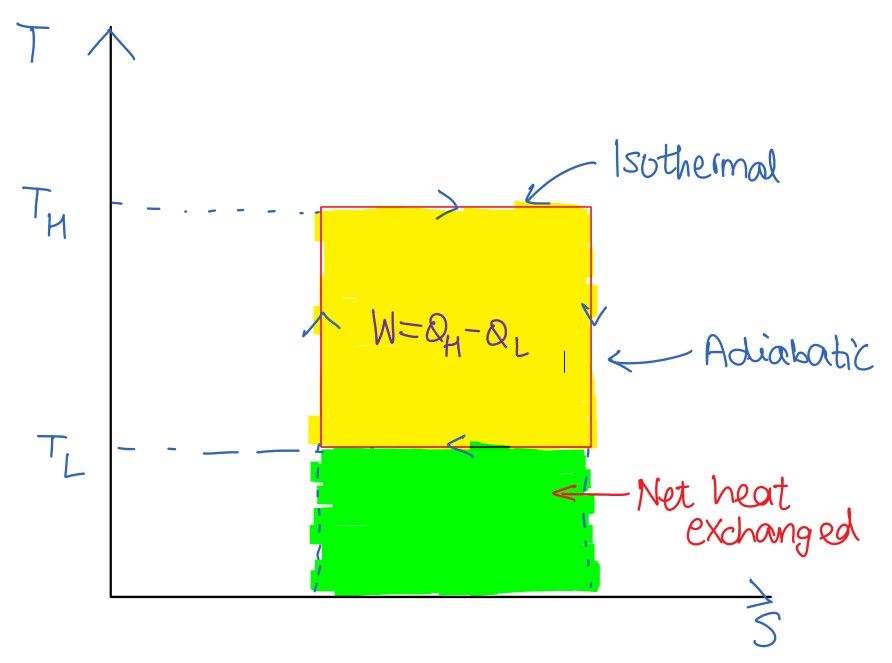
\includegraphics[scale=0.6]{clausius3.jpg}
	\centering
\end{figure}

\section{Entropy Calculations}

\subsection{Dependence of entropy on temperature}
\begin{equation}
	\boxed{\Delta S_v=S_2-S_1=\int_{T_1}^{T_2}C_v d(\ln T)}\qq{at constant volume.}
\end{equation}
\begin{equation}
	\boxed{\Delta S_p=S_2-S_1=\int_{T_1}^{T_2}C_p d(\ln T)}\qq{at constant pressure.}
\end{equation}
\subsection{Dependence of entropy on volume}
\begin{equation}
	dS=\frac{1}{T}\Bigg(\pdv{U}{T}\Bigg)_VdT+\Bigg(\pdv{P}{T}\Bigg)_V dV.
\end{equation}
Under isothermal conditions we will get
\begin{equation}
	dS_T=\Bigg(\pdv{P}{T}\Bigg)_VdV
\end{equation}
From the reciprocity relation we get,
\begin{equation}
	\boxed{dS_T=\frac{\alpha}{\beta}dV}
\end{equation}

\subsection{Dependence of entropy on pressure}
\begin{equation}
		dS=\frac{1}{T}\Bigg(\pdv{H}{T}\Bigg)_PdT+\Bigg(\pdv{V}{T}\Bigg)_P dP.
\end{equation}

\begin{equation}
	\boxed{dS_T=-\alpha VdP}
\end{equation}

\subsection{Relation between $C_p$ \& $C_v$ 2.0}
\begin{equation}
	\boxed{C_p-C_v=\dfrac{\alpha^2 VT}{\beta}}
\end{equation}
Analogues of Hess's law and Kirchoff's law are applicable for entropy as well. The only differences being that exact value of entropy can be determined and entropy is only calculated in a reversible process(since entropy is a state function).

\subsection{Entropy change in phase transformations}
\begin{equation}
	\Delta S_{tr}^{0}=\dfrac{\Delta H_{tr}^{0}}{T_{tr}}
\end{equation}

\begin{tcolorbox}[title=Example]
	\ce{A_{(s)}(298 K) -> A_{(l)}(T_mK) -> A_{g}(TK)}
	\tcblower
	\begin{equation*}
		S_{T}^{0}-S_{298}^{0}=\int_{298}^{T_m}\frac{C_p\text{(solid)}}{T}dT + \frac{\Delta H_m}{T_m} + \int_{T_m}^{T_b}\frac{C_p(\text{(liq.)}}{T}dT + \frac{\Delta H_b}{T_b} + \int_{T_b}^{T}\frac{C_p\text{(gas)}}{T}dT
	\end{equation*}
\end{tcolorbox}

\section{Thermodynamic Potentials}
\begin{align*}
	dS&=\frac{dQ_{rev}}{T} \\
   dU&=dQ-PdV\\
   dU&=TdS-PdV\\
   TdS&=dU+PdV\\
\end{align*}
So we can say that for a spontaneous process
\begin{align}
	TdS&>dU+PdV\\
	&\qq{and for an unnatural process} \\
	TdS&<dU+PdV.
\end{align}
If the system moves from one state to the other then there must be some driving force for the process to take place and is called the thermodynamic potential. For e.g. if gas is effusing due to a higher pressure one side then the mechanical potential is at play. In case of an electric field a charge moves from higher to lower potential. So in general a system moves from higher to lower potential. Enthalpy, internal energy and entropy are thermodynamic potentials. If a system goes from higher $S$ to a lower $S$ then we will say that the process is entropy driven. Same goes for any thermodynamic potential. 
\paragraph*{Examples}
\begin{enumerate}
	\item \ce{C(s) + O2(g) -> CO2(g)} \quad: $\Delta H_{298}=-94050$ cal/mol. So this process is enthalpy driven, so can we conclude that the fate of each system can be determined by enthalpy?
	\item \ce{ZnO(s) + C(s) -> Zn(g)+CO(g)} \quad: $\Delta H_{1373}=83200$ cal/mol but $ \Delta S=1371 $ cal/mol*degree. This reaction is non spontaneous below the melting point of zinc but after the melting point it is entropy driven. So is entropy a sufficient condition for determining the spontaneity of a process? 
	\item \ce{Fe(s) +1/2 O2(g) -> FeO(s)}\quad: $\Delta S=-17$ cal/deg  however iron oxidises spontaneously. 
	
\end{enumerate}
We can conclude that the spontaneity of a process depends on the \textit{quantity} and \textit{quality} of the energy in the system and how the two change.







\end{document}